%%  ************    LibreSilicon's 1st TestWafer    *******************
%%
%%  Organisation:   Chipforge
%%                  Germany / European Union
%%
%%  Profile:        Chipforge focus on fine System-on-Chip Cores in
%%                  Verilog HDL Code which are easy understandable and
%%                  adjustable. For further information see
%%                          www.chipforge.org
%%                  there are projects from small cores up to PCBs, too.
%%
%%  File:           PearlRiver/Documents/LaTeX/die_quarter.tex
%%
%%  Purpose:        Principle Description Pictgure for quarters
%%
%%  ************    LaTeX with circdia.sty package      ***************
%%
%%  ///////////////////////////////////////////////////////////////////
%%
%%  Copyright (c) 2018 by chipforge <hsank@nospam.chipforge.org>
%%  All rights reserved.
%%
%%      This Standard Cell Library is licensed under the Libre Silicon
%%      public license; you can redistribute it and/or modify it under
%%      the terms of the Libre Silicon public license as published by
%%      the Libre Silicon alliance, either version 1 of the License, or
%%      (at your option) any later version.
%%
%%      This design is distributed in the hope that it will be useful,
%%      but WITHOUT ANY WARRANTY; without even the implied warranty of
%%      MERCHANTABILITY or FITNESS FOR A PARTICULAR PURPOSE.
%%      See the Libre Silicon Public License for more details.
%%
%%  ///////////////////////////////////////////////////////////////////
\begin{center}
    Principle - $R_\square$
    \begin{figure}[h]
        \begin{center}
            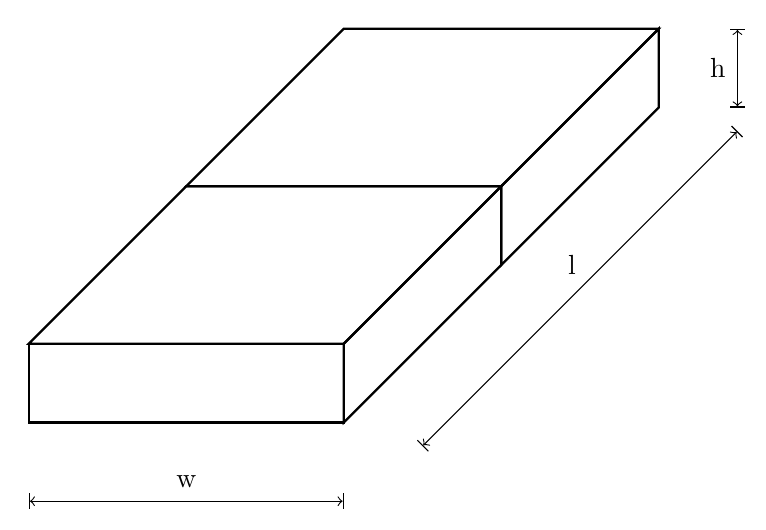
\begin{tikzpicture}[]
            \draw[thick] (0,0) -- (4,0) -- (4,1) -- (0,1) -- cycle; % front
            \draw[thick] (0,1) -- (2,3) -- (6,3) -- (4,1) -- cycle; % 1st top
            \draw[thick] (4,0) -- (4,1) -- (6,3) -- (6,2) -- cycle; % 1st boarder
            \draw[thick] (2,3) -- (4,5) -- (8,5) -- (6,3) -- cycle; % 2nd top
            \draw[thick] (6,3) -- (8,5) -- (8,4) -- (6,2) -- cycle; % 2nd boarder
            % width
            \node at (2,-0.75) {w};
            \draw[|<->|] (0,-1) -- (4,-1);
            % length
            \node at (6.9,2) {l};
            \draw[|<->|] (5,-0.3) -- (9,3.7);
            % hight
            \node at (8.75,4.5) {h};
            \draw[|<->|] (9,4) -- (9,5);
            \end{tikzpicture}
        \end{center}
    \end{figure}
\end{center}
